\documentclass[11pt]{amsart}
\usepackage{geometry} % see geometry.pdf on how to lay out the page. There's lots.
\geometry{a4paper} % or letter or a5paper or ... etc
% \geometry{landscape} % rotated page geometry
\usepackage{amsmath}
\usepackage{graphicx}
\usepackage{breqn}

\setcounter{MaxMatrixCols}{10}

\flushbottom
\chardef\atcode=\catcode`\@
\makeatletter
\@addtoreset{figure}{section}
\@addtoreset{table}{section}
\renewcommand{\figurename}{Figure}
\renewcommand{\tablename}{Table}
\setcounter{topnumber}{3}               % orig: 2
\setcounter{totalnumber}{4}             % orig: 3
\renewcommand{\textfraction}{0}         
\renewcommand{\bottomfraction}{0.65}    
\renewcommand{\topfraction}{0.75}       
\renewcommand{\floatpagefraction}{0.75} 
\catcode`\@=\atcode 
\newcommand{\grad}{$^\circ$}
\newcommand{\gradm}{^\circ}
\newcommand{\bqn}{ \begin{eqnarray} }
\newcommand{\eqn}{ \end{eqnarray} }
\newcommand{\beq}{ \begin{equation} }
\newcommand{\eeq}{ \end{equation} }
\setlength{\baselineskip}{2.1ex}
\renewcommand{\baselinestretch}{1.06}
\setlength{\parskip}{1.5ex plus 0.8ex minus 0.6ex}
\setlength{\evensidemargin}{0.3cm}
\setlength{\oddsidemargin}{0.2cm}
\setlength{\topmargin}{-1cm}
\setlength{\textwidth}{16.5cm}
\setlength{\textheight}{26cm}
\newcommand{\mat}[1]{\mbox{$\underline{\underline{#1}}$}}
\newcommand{\etal}{\mbox{\sl et al.}}
\renewcommand{\refname}{}
\newcommand{\vol}[1]{{\bf{#1}}}
\newcommand{\dg}{$^\circ\;$}
\def\D{\displaystyle}
\newcommand{\lapprox}{\ensuremath{<\atop{\mbox{\raisebox{0.5ex}{$\sim$}}}}}
\parindent 0cm
% Macros for Scientific Word 2.5 documents saved with the LaTeX filter.
%Copyright (C) 1994-95 TCI Software Research, Inc.
\typeout{TCILATEX Macros for Scientific Word 2.5 <22 Dec 95>.}
\typeout{NOTICE:  This macro file is NOT proprietary and may be 
freely copied and distributed.}
%
\makeatletter
%
%%%%%%%%%%%%%%%%%%%%%%
% macros for time
\newcount\@hour\newcount\@minute\chardef\@x10\chardef\@xv60
\def\tcitime{
\def\@time{%
  \@minute\time\@hour\@minute\divide\@hour\@xv
  \ifnum\@hour<\@x 0\fi\the\@hour:%
  \multiply\@hour\@xv\advance\@minute-\@hour
  \ifnum\@minute<\@x 0\fi\the\@minute
  }}%

%%%%%%%%%%%%%%%%%%%%%%
% macro for hyperref
\@ifundefined{hyperref}{\def\hyperref#1#2#3#4{#2\ref{#4}#3}}{}

% macro for external program call
\@ifundefined{qExtProgCall}{\def\qExtProgCall#1#2#3#4#5#6{\relax}}{}
%%%%%%%%%%%%%%%%%%%%%%
%
% macros for graphics
%
\def\FILENAME#1{#1}%
%
\def\QCTOpt[#1]#2{%
  \def\QCTOptB{#1}
  \def\QCTOptA{#2}
}
\def\QCTNOpt#1{%
  \def\QCTOptA{#1}
  \let\QCTOptB\empty
}
\def\Qct{%
  \@ifnextchar[{%
    \QCTOpt}{\QCTNOpt}
}
\def\QCBOpt[#1]#2{%
  \def\QCBOptB{#1}
  \def\QCBOptA{#2}
}
\def\QCBNOpt#1{%
  \def\QCBOptA{#1}
  \let\QCBOptB\empty
}
\def\Qcb{%
  \@ifnextchar[{%
    \QCBOpt}{\QCBNOpt}
}
\def\PrepCapArgs{%
  \ifx\QCBOptA\empty
    \ifx\QCTOptA\empty
      {}%
    \else
      \ifx\QCTOptB\empty
        {\QCTOptA}%
      \else
        [\QCTOptB]{\QCTOptA}%
      \fi
    \fi
  \else
    \ifx\QCBOptA\empty
      {}%
    \else
      \ifx\QCBOptB\empty
        {\QCBOptA}%
      \else
        [\QCBOptB]{\QCBOptA}%
      \fi
    \fi
  \fi
}
\newcount\GRAPHICSTYPE
%\GRAPHICSTYPE 0 is for TurboTeX
%\GRAPHICSTYPE 1 is for DVIWindo (PostScript)
%%%(removed)%\GRAPHICSTYPE 2 is for psfig (PostScript)
\GRAPHICSTYPE=\z@
\def\GRAPHICSPS#1{%
 \ifcase\GRAPHICSTYPE%\GRAPHICSTYPE=0
   \special{ps: #1}%
 \or%\GRAPHICSTYPE=1
   \special{language "PS", include "#1"}%
%%%\or%\GRAPHICSTYPE=2
%%%  #1%
 \fi
}%
%
\def\GRAPHICSHP#1{\special{include #1}}%
%
% \graffile{ body }                                  %#1
%          { contentswidth (scalar)  }               %#2
%          { contentsheight (scalar) }               %#3
%          { vertical shift when in-line (scalar) }  %#4
\def\graffile#1#2#3#4{%
%%% \ifnum\GRAPHICSTYPE=\tw@
%%%  %Following if using psfig
%%%  \@ifundefined{psfig}{\input psfig.tex}{}%
%%%  \psfig{file=#1, height=#3, width=#2}%
%%% \else
  %Following for all others
  % JCS - added BOXTHEFRAME, see below
    \leavevmode
    \raise -#4 \BOXTHEFRAME{%
        \hbox to #2{\raise #3\hbox to #2{\null #1\hfil}}}%
}%
%
% A box for drafts
\def\draftbox#1#2#3#4{%
 \leavevmode\raise -#4 \hbox{%
  \frame{\rlap{\protect\tiny #1}\hbox to #2%
   {\vrule height#3 width\z@ depth\z@\hfil}%
  }%
 }%
}%
%
\newcount\draft
\draft=\z@
\let\nographics=\draft
\newif\ifwasdraft
\wasdraftfalse

%  \GRAPHIC{ body }                                  %#1
%          { draft name }                            %#2
%          { contentswidth (scalar)  }               %#3
%          { contentsheight (scalar) }               %#4
%          { vertical shift when in-line (scalar) }  %#5
\def\GRAPHIC#1#2#3#4#5{%
 \ifnum\draft=\@ne\draftbox{#2}{#3}{#4}{#5}%
  \else\graffile{#1}{#3}{#4}{#5}%
  \fi
 }%
%
\def\addtoLaTeXparams#1{%
    \edef\LaTeXparams{\LaTeXparams #1}}%
%
% JCS -  added a switch BoxFrame that can 
% be set by including X in the frame params.
% If set a box is drawn around the frame.

\newif\ifBoxFrame \BoxFramefalse
\newif\ifOverFrame \OverFramefalse
\newif\ifUnderFrame \UnderFramefalse

\def\BOXTHEFRAME#1{%
   \hbox{%
      \ifBoxFrame
         \frame{#1}%
      \else
         {#1}%
      \fi
   }%
}


\def\doFRAMEparams#1{\BoxFramefalse\OverFramefalse\UnderFramefalse\readFRAMEparams#1\end}%
\def\readFRAMEparams#1{%
 \ifx#1\end%
  \let\next=\relax
  \else
  \ifx#1i\dispkind=\z@\fi
  \ifx#1d\dispkind=\@ne\fi
  \ifx#1f\dispkind=\tw@\fi
  \ifx#1t\addtoLaTeXparams{t}\fi
  \ifx#1b\addtoLaTeXparams{b}\fi
  \ifx#1p\addtoLaTeXparams{p}\fi
  \ifx#1h\addtoLaTeXparams{h}\fi
  \ifx#1X\BoxFrametrue\fi
  \ifx#1O\OverFrametrue\fi
  \ifx#1U\UnderFrametrue\fi
  \ifx#1w
    \ifnum\draft=1\wasdrafttrue\else\wasdraftfalse\fi
    \draft=\@ne
  \fi
  \let\next=\readFRAMEparams
  \fi
 \next
 }%
%
%Macro for In-line graphics object
%   \IFRAME{ contentswidth (scalar)  }               %#1
%          { contentsheight (scalar) }               %#2
%          { vertical shift when in-line (scalar) }  %#3
%          { draft name }                            %#4
%          { body }                                  %#5
%          { caption}                                %#6


\def\IFRAME#1#2#3#4#5#6{%
      \bgroup
      \let\QCTOptA\empty
      \let\QCTOptB\empty
      \let\QCBOptA\empty
      \let\QCBOptB\empty
      #6%
      \parindent=0pt%
      \leftskip=0pt
      \rightskip=0pt
      \setbox0 = \hbox{\QCBOptA}%
      \@tempdima = #1\relax
      \ifOverFrame
          % Do this later
          \typeout{This is not implemented yet}%
          \show\HELP
      \else
         \ifdim\wd0>\@tempdima
            \advance\@tempdima by \@tempdima
            \ifdim\wd0 >\@tempdima
               \textwidth=\@tempdima
               \setbox1 =\vbox{%
                  \noindent\hbox to \@tempdima{\hfill\GRAPHIC{#5}{#4}{#1}{#2}{#3}\hfill}\\%
                  \noindent\hbox to \@tempdima{\parbox[b]{\@tempdima}{\QCBOptA}}%
               }%
               \wd1=\@tempdima
            \else
               \textwidth=\wd0
               \setbox1 =\vbox{%
                 \noindent\hbox to \wd0{\hfill\GRAPHIC{#5}{#4}{#1}{#2}{#3}\hfill}\\%
                 \noindent\hbox{\QCBOptA}%
               }%
               \wd1=\wd0
            \fi
         \else
            %\show\BBB
            \ifdim\wd0>0pt
              \hsize=\@tempdima
              \setbox1 =\vbox{%
                \unskip\GRAPHIC{#5}{#4}{#1}{#2}{0pt}%
                \break
                \unskip\hbox to \@tempdima{\hfill \QCBOptA\hfill}%
              }%
              \wd1=\@tempdima
           \else
              \hsize=\@tempdima
              \setbox1 =\vbox{%
                \unskip\GRAPHIC{#5}{#4}{#1}{#2}{0pt}%
              }%
              \wd1=\@tempdima
           \fi
         \fi
         \@tempdimb=\ht1
         \advance\@tempdimb by \dp1
         \advance\@tempdimb by -#2%
         \advance\@tempdimb by #3%
         \leavevmode
         \raise -\@tempdimb \hbox{\box1}%
      \fi
      \egroup%
}%
%
%Macro for Display graphics object
%   \DFRAME{ contentswidth (scalar)  }               %#1
%          { contentsheight (scalar) }               %#2
%          { draft label }                           %#3
%          { name }                                  %#4
%          { caption}                                %#5
\def\DFRAME#1#2#3#4#5{%
 \begin{center}
     \let\QCTOptA\empty
     \let\QCTOptB\empty
     \let\QCBOptA\empty
     \let\QCBOptB\empty
     \ifOverFrame 
        #5\QCTOptA\par
     \fi
     \GRAPHIC{#4}{#3}{#1}{#2}{\z@}
     \ifUnderFrame 
        \nobreak\par #5\QCBOptA
     \fi
 \end{center}%
 }%
%
%Macro for Floating graphic object
%   \FFRAME{ framedata f|i tbph x F|T }              %#1
%          { contentswidth (scalar)  }               %#2
%          { contentsheight (scalar) }               %#3
%          { caption }                               %#4
%          { label }                                 %#5
%          { draft name }                            %#6
%          { body }                                  %#7
\def\FFRAME#1#2#3#4#5#6#7{%
 \begin{figure}[#1]%
  \let\QCTOptA\empty
  \let\QCTOptB\empty
  \let\QCBOptA\empty
  \let\QCBOptB\empty
  \ifOverFrame
    #4
    \ifx\QCTOptA\empty
    \else
      \ifx\QCTOptB\empty
        \caption{\QCTOptA}%
      \else
        \caption[\QCTOptB]{\QCTOptA}%
      \fi
    \fi
    \ifUnderFrame\else
      \label{#5}%
    \fi
  \else
    \UnderFrametrue%
  \fi
  \begin{center}\GRAPHIC{#7}{#6}{#2}{#3}{\z@}\end{center}%
  \ifUnderFrame
    #4
    \ifx\QCBOptA\empty
      \caption{}%
    \else
      \ifx\QCBOptB\empty
        \caption{\QCBOptA}%
      \else
        \caption[\QCBOptB]{\QCBOptA}%
      \fi
    \fi
    \label{#5}%
  \fi
  \end{figure}%
 }%
%
%
%    \FRAME{ framedata f|i tbph x F|T }              %#1
%          { contentswidth (scalar)  }               %#2
%          { contentsheight (scalar) }               %#3
%          { vertical shift when in-line (scalar) }  %#4
%          { caption }                               %#5
%          { label }                                 %#6
%          { name }                                  %#7
%          { body }                                  %#8
%
%    framedata is a string which can contain the following
%    characters: idftbphxFT
%    Their meaning is as follows:
%             i, d or f : in-line, display, or floating
%             t,b,p,h   : LaTeX floating placement options
%             x         : fit contents box to contents
%             F or T    : Figure or Table. 
%                         Later this can expand
%                         to a more general float class.
%
%
\newcount\dispkind%

\def\makeactives{
  \catcode`\"=\active
  \catcode`\;=\active
  \catcode`\:=\active
  \catcode`\'=\active
  \catcode`\~=\active
}
\bgroup
   \makeactives
   \gdef\activesoff{%
      \def"{\string"}
      \def;{\string;}
      \def:{\string:}
      \def'{\string'}
      \def~{\string~}
      %\bbl@deactivate{"}%
      %\bbl@deactivate{;}%
      %\bbl@deactivate{:}%
      %\bbl@deactivate{'}%
    }
\egroup

\def\FRAME#1#2#3#4#5#6#7#8{%
 \bgroup
 \@ifundefined{bbl@deactivate}{}{\activesoff}
 \ifnum\draft=\@ne
   \wasdrafttrue
 \else
   \wasdraftfalse%
 \fi
 \def\LaTeXparams{}%
 \dispkind=\z@
 \def\LaTeXparams{}%
 \doFRAMEparams{#1}%
 \ifnum\dispkind=\z@\IFRAME{#2}{#3}{#4}{#7}{#8}{#5}\else
  \ifnum\dispkind=\@ne\DFRAME{#2}{#3}{#7}{#8}{#5}\else
   \ifnum\dispkind=\tw@
    \edef\@tempa{\noexpand\FFRAME{\LaTeXparams}}%
    \@tempa{#2}{#3}{#5}{#6}{#7}{#8}%
    \fi
   \fi
  \fi
  \ifwasdraft\draft=1\else\draft=0\fi{}%
  \egroup
 }%
%
% This macro added to let SW gobble a parameter that
% should not be passed on and expanded. 

\def\TEXUX#1{"texux"}

%
% Macros for text attributes:
%
\def\BF#1{{\bf {#1}}}%
\def\NEG#1{\leavevmode\hbox{\rlap{\thinspace/}{$#1$}}}%
%
%%%%%%%%%%%%%%%%%%%%%%%%%%%%%%%%%%%%%%%%%%%%%%%%%%%%%%%%%%%%%%%%%%%%%%%%
%
%
% macros for user - defined functions
\def\func#1{\mathop{\rm #1}}%
\def\limfunc#1{\mathop{\rm #1}}%

%
% miscellaneous 
%\long\def\QQQ#1#2{}%
\long\def\QQQ#1#2{%
     \long\expandafter\def\csname#1\endcsname{#2}}%
%\def\QTP#1{}% JCS - this was changed becuase style editor will define QTP
\@ifundefined{QTP}{\def\QTP#1{}}{}
\@ifundefined{QEXCLUDE}{\def\QEXCLUDE#1{}}{}
%\@ifundefined{Qcb}{\def\Qcb#1{#1}}{}
%\@ifundefined{Qct}{\def\Qct#1{#1}}{}
\@ifundefined{Qlb}{\def\Qlb#1{#1}}{}
\@ifundefined{Qlt}{\def\Qlt#1{#1}}{}
\def\QWE{}%
\long\def\QQA#1#2{}%
%\def\QTR#1#2{{\em #2}}% Always \em!!!
%\def\QTR#1#2{\mbox{\begin{#1}#2\end{#1}}}%cb%%%
\def\QTR#1#2{{\csname#1\endcsname #2}}%(gp) Is this the best?
\long\def\TeXButton#1#2{#2}%
\long\def\QSubDoc#1#2{#2}%
\def\EXPAND#1[#2]#3{}%
\def\NOEXPAND#1[#2]#3{}%
\def\PROTECTED{}%
\def\LaTeXparent#1{}%
\def\ChildStyles#1{}%
\def\ChildDefaults#1{}%
\def\QTagDef#1#2#3{}%
%
% Macros for style editor docs
\@ifundefined{StyleEditBeginDoc}{\def\StyleEditBeginDoc{\relax}}{}
%
% Macros for footnotes
\def\QQfnmark#1{\footnotemark}
\def\QQfntext#1#2{\addtocounter{footnote}{#1}\footnotetext{#2}}
%
% Macros for indexing.
\def\MAKEINDEX{\makeatletter\input gnuindex.sty\makeatother\makeindex}%	
\@ifundefined{INDEX}{\def\INDEX#1#2{}{}}{}%
\@ifundefined{SUBINDEX}{\def\SUBINDEX#1#2#3{}{}{}}{}%
\@ifundefined{initial}%  
   {\def\initial#1{\bigbreak{\raggedright\large\bf #1}\kern 2\p@\penalty3000}}%
   {}%
\@ifundefined{entry}{\def\entry#1#2{\item {#1}, #2}}{}%
\@ifundefined{primary}{\def\primary#1{\item {#1}}}{}%
\@ifundefined{secondary}{\def\secondary#1#2{\subitem {#1}, #2}}{}%
%
%
\@ifundefined{ZZZ}{}{\MAKEINDEX\makeatletter}%
%
% Attempts to avoid problems with other styles
\@ifundefined{abstract}{%
 \def\abstract{%
  \if@twocolumn
   \section*{Abstract (Not appropriate in this style!)}%
   \else \small 
   \begin{center}{\bf Abstract\vspace{-.5em}\vspace{\z@}}\end{center}%
   \quotation 
   \fi
  }%
 }{%
 }%
\@ifundefined{endabstract}{\def\endabstract
  {\if@twocolumn\else\endquotation\fi}}{}%
\@ifundefined{maketitle}{\def\maketitle#1{}}{}%
\@ifundefined{affiliation}{\def\affiliation#1{}}{}%
\@ifundefined{proof}{\def\proof{\noindent{\bfseries Proof. }}}{}%
\@ifundefined{endproof}{\def\endproof{\mbox{\ \rule{.1in}{.1in}}}}{}%
\@ifundefined{newfield}{\def\newfield#1#2{}}{}%
\@ifundefined{chapter}{\def\chapter#1{\par(Chapter head:)#1\par }%
 \newcount\c@chapter}{}%
\@ifundefined{part}{\def\part#1{\par(Part head:)#1\par }}{}%
\@ifundefined{section}{\def\section#1{\par(Section head:)#1\par }}{}%
\@ifundefined{subsection}{\def\subsection#1%
 {\par(Subsection head:)#1\par }}{}%
\@ifundefined{subsubsection}{\def\subsubsection#1%
 {\par(Subsubsection head:)#1\par }}{}%
\@ifundefined{paragraph}{\def\paragraph#1%
 {\par(Subsubsubsection head:)#1\par }}{}%
\@ifundefined{subparagraph}{\def\subparagraph#1%
 {\par(Subsubsubsubsection head:)#1\par }}{}%
%%%%%%%%%%%%%%%%%%%%%%%%%%%%%%%%%%%%%%%%%%%%%%%%%%%%%%%%%%%%%%%%%%%%%%%%
% These symbols are not recognized by LaTeX
\@ifundefined{therefore}{\def\therefore{}}{}%
\@ifundefined{backepsilon}{\def\backepsilon{}}{}%
\@ifundefined{yen}{\def\yen{\hbox{\rm\rlap=Y}}}{}%
\@ifundefined{registered}{%
   \def\registered{\relax\ifmmode{}\r@gistered
                    \else$\m@th\r@gistered$\fi}%
 \def\r@gistered{^{\ooalign
  {\hfil\raise.07ex\hbox{$\scriptstyle\rm\text{R}$}\hfil\crcr
  \mathhexbox20D}}}}{}%
\@ifundefined{Eth}{\def\Eth{}}{}%
\@ifundefined{eth}{\def\eth{}}{}%
\@ifundefined{Thorn}{\def\Thorn{}}{}%
\@ifundefined{thorn}{\def\thorn{}}{}%
% A macro to allow any symbol that requires math to appear in text
\def\TEXTsymbol#1{\mbox{$#1$}}%
\@ifundefined{degree}{\def\degree{{}^{\circ}}}{}%
%
% macros for T3TeX files
\newdimen\theight
\def\Column{%
 \vadjust{\setbox\z@=\hbox{\scriptsize\quad\quad tcol}%
  \theight=\ht\z@\advance\theight by \dp\z@\advance\theight by \lineskip
  \kern -\theight \vbox to \theight{%
   \rightline{\rlap{\box\z@}}%
   \vss
   }%
  }%
 }%
%
\def\qed{%
 \ifhmode\unskip\nobreak\fi\ifmmode\ifinner\else\hskip5\p@\fi\fi
 \hbox{\hskip5\p@\vrule width4\p@ height6\p@ depth1.5\p@\hskip\p@}%
 }%
%
\def\cents{\hbox{\rm\rlap/c}}%
\def\miss{\hbox{\vrule height2\p@ width 2\p@ depth\z@}}%
%\def\miss{\hbox{.}}%        %another possibility 
%
\def\vvert{\Vert}%           %always translated to \left| or \right|
%
\def\tcol#1{{\baselineskip=6\p@ \vcenter{#1}} \Column}  %
%
\def\dB{\hbox{{}}}%                 %dummy entry in column 
\def\mB#1{\hbox{$#1$}}%             %column entry
\def\nB#1{\hbox{#1}}%               %column entry (not math)
%
%\newcount\notenumber
%\def\clearnotenumber{\notenumber=0}
%\def\note{\global\advance\notenumber by 1
% \footnote{$^{\the\notenumber}$}}
%\def\note{\global\advance\notenumber by 1
\def\note{$^{\dag}}%
%
%

\def\newfmtname{LaTeX2e}
\def\chkcompat{%
   \if@compatibility
   \else
     \usepackage{latexsym}
   \fi
}

\ifx\fmtname\newfmtname
  \DeclareOldFontCommand{\rm}{\normalfont\rmfamily}{\mathrm}
  \DeclareOldFontCommand{\sf}{\normalfont\sffamily}{\mathsf}
  \DeclareOldFontCommand{\tt}{\normalfont\ttfamily}{\mathtt}
  \DeclareOldFontCommand{\bf}{\normalfont\bfseries}{\mathbf}
  \DeclareOldFontCommand{\it}{\normalfont\itshape}{\mathit}
  \DeclareOldFontCommand{\sl}{\normalfont\slshape}{\@nomath\sl}
  \DeclareOldFontCommand{\sc}{\normalfont\scshape}{\@nomath\sc}
  \chkcompat
\fi

%
% Greek bold macros
% Redefine all of the math symbols 
% which might be bolded	 - there are 
% probably others to add to this list

\def\alpha{\Greekmath 010B }%
\def\beta{\Greekmath 010C }%
\def\gamma{\Greekmath 010D }%
\def\delta{\Greekmath 010E }%
\def\epsilon{\Greekmath 010F }%
\def\zeta{\Greekmath 0110 }%
\def\eta{\Greekmath 0111 }%
\def\theta{\Greekmath 0112 }%
\def\iota{\Greekmath 0113 }%
\def\kappa{\Greekmath 0114 }%
\def\lambda{\Greekmath 0115 }%
\def\mu{\Greekmath 0116 }%
\def\nu{\Greekmath 0117 }%
\def\xi{\Greekmath 0118 }%
\def\pi{\Greekmath 0119 }%
\def\rho{\Greekmath 011A }%
\def\sigma{\Greekmath 011B }%
\def\tau{\Greekmath 011C }%
\def\upsilon{\Greekmath 011D }%
\def\phi{\Greekmath 011E }%
\def\chi{\Greekmath 011F }%
\def\psi{\Greekmath 0120 }%
\def\omega{\Greekmath 0121 }%
\def\varepsilon{\Greekmath 0122 }%
\def\vartheta{\Greekmath 0123 }%
\def\varpi{\Greekmath 0124 }%
\def\varrho{\Greekmath 0125 }%
\def\varsigma{\Greekmath 0126 }%
\def\varphi{\Greekmath 0127 }%

\def\nabla{\Greekmath 0272 }
\def\FindBoldGroup{%
   {\setbox0=\hbox{$\mathbf{x\global\edef\theboldgroup{\the\mathgroup}}$}}%
}

\def\Greekmath#1#2#3#4{%
    \if@compatibility
        \ifnum\mathgroup=\symbold
           \mathchoice{\mbox{\boldmath$\displaystyle\mathchar"#1#2#3#4$}}%
                      {\mbox{\boldmath$\textstyle\mathchar"#1#2#3#4$}}%
                      {\mbox{\boldmath$\scriptstyle\mathchar"#1#2#3#4$}}%
                      {\mbox{\boldmath$\scriptscriptstyle\mathchar"#1#2#3#4$}}%
        \else
           \mathchar"#1#2#3#4% 
        \fi 
    \else 
        \FindBoldGroup
        \ifnum\mathgroup=\theboldgroup % For 2e
           \mathchoice{\mbox{\boldmath$\displaystyle\mathchar"#1#2#3#4$}}%
                      {\mbox{\boldmath$\textstyle\mathchar"#1#2#3#4$}}%
                      {\mbox{\boldmath$\scriptstyle\mathchar"#1#2#3#4$}}%
                      {\mbox{\boldmath$\scriptscriptstyle\mathchar"#1#2#3#4$}}%
        \else
           \mathchar"#1#2#3#4% 
        \fi     	    
	  \fi}

\newif\ifGreekBold  \GreekBoldfalse
\let\SAVEPBF=\pbf
\def\pbf{\GreekBoldtrue\SAVEPBF}%
%

\@ifundefined{theorem}{\newtheorem{theorem}{Theorem}}{}
\@ifundefined{lemma}{\newtheorem{lemma}[theorem]{Lemma}}{}
\@ifundefined{corollary}{\newtheorem{corollary}[theorem]{Corollary}}{}
\@ifundefined{conjecture}{\newtheorem{conjecture}[theorem]{Conjecture}}{}
\@ifundefined{proposition}{\newtheorem{proposition}[theorem]{Proposition}}{}
\@ifundefined{axiom}{\newtheorem{axiom}{Axiom}}{}
\@ifundefined{remark}{\newtheorem{remark}{Remark}}{}
\@ifundefined{example}{\newtheorem{example}{Example}}{}
\@ifundefined{exercise}{\newtheorem{exercise}{Exercise}}{}
\@ifundefined{definition}{\newtheorem{definition}{Definition}}{}


\@ifundefined{mathletters}{%
  %\def\theequation{\arabic{equation}}
  \newcounter{equationnumber}  
  \def\mathletters{%
     \addtocounter{equation}{1}
     \edef\@currentlabel{\theequation}%
     \setcounter{equationnumber}{\c@equation}
     \setcounter{equation}{0}%
     \edef\theequation{\@currentlabel\noexpand\alph{equation}}%
  }
  \def\endmathletters{%
     \setcounter{equation}{\value{equationnumber}}%
  }
}{}

%Logos
\@ifundefined{BibTeX}{%
    \def\BibTeX{{\rm B\kern-.05em{\sc i\kern-.025em b}\kern-.08em
                 T\kern-.1667em\lower.7ex\hbox{E}\kern-.125emX}}}{}%
\@ifundefined{AmS}%
    {\def\AmS{{\protect\usefont{OMS}{cmsy}{m}{n}%
                A\kern-.1667em\lower.5ex\hbox{M}\kern-.125emS}}}{}%
\@ifundefined{AmSTeX}{\def\AmSTeX{\protect\AmS-\protect\TeX\@}}{}%
%

%%%%%%%%%%%%%%%%%%%%%%%%%%%%%%%%%%%%%%%%%%%%%%%%%%%%%%%%%%%%%%%%%%%%%%%
% NOTE: The rest of this file is read only if amstex has not been
% loaded.  This section is used to define amstex constructs in the
% event they have not been defined.
%
%
\ifx\ds@amstex\relax
   \message{amstex already loaded}\makeatother\endinput% 2.09 compatability
\else
   \@ifpackageloaded{amstex}%
      {\message{amstex already loaded}\makeatother\endinput}
      {}
   \@ifpackageloaded{amsgen}%
      {\message{amsgen already loaded}\makeatother\endinput}
      {}
\fi
%%%%%%%%%%%%%%%%%%%%%%%%%%%%%%%%%%%%%%%%%%%%%%%%%%%%%%%%%%%%%%%%%%%%%%%%
%%
%
%
%  Macros to define some AMS LaTeX constructs when 
%  AMS LaTeX has not been loaded
% 
% These macros are copied from the AMS-TeX package for doing
% multiple integrals.
%
\let\DOTSI\relax
\def\RIfM@{\relax\ifmmode}%
\def\FN@{\futurelet\next}%
\newcount\intno@
\def\iint{\DOTSI\intno@\tw@\FN@\ints@}%
\def\iiint{\DOTSI\intno@\thr@@\FN@\ints@}%
\def\iiiint{\DOTSI\intno@4 \FN@\ints@}%
\def\idotsint{\DOTSI\intno@\z@\FN@\ints@}%
\def\ints@{\findlimits@\ints@@}%
\newif\iflimtoken@
\newif\iflimits@
\def\findlimits@{\limtoken@true\ifx\next\limits\limits@true
 \else\ifx\next\nolimits\limits@false\else
 \limtoken@false\ifx\ilimits@\nolimits\limits@false\else
 \ifinner\limits@false\else\limits@true\fi\fi\fi\fi}%
\def\multint@{\int\ifnum\intno@=\z@\intdots@                          %1
 \else\intkern@\fi                                                    %2
 \ifnum\intno@>\tw@\int\intkern@\fi                                   %3
 \ifnum\intno@>\thr@@\int\intkern@\fi                                 %4
 \int}%                                                               %5
\def\multintlimits@{\intop\ifnum\intno@=\z@\intdots@\else\intkern@\fi
 \ifnum\intno@>\tw@\intop\intkern@\fi
 \ifnum\intno@>\thr@@\intop\intkern@\fi\intop}%
\def\intic@{%
    \mathchoice{\hskip.5em}{\hskip.4em}{\hskip.4em}{\hskip.4em}}%
\def\negintic@{\mathchoice
 {\hskip-.5em}{\hskip-.4em}{\hskip-.4em}{\hskip-.4em}}%
\def\ints@@{\iflimtoken@                                              %1
 \def\ints@@@{\iflimits@\negintic@
   \mathop{\intic@\multintlimits@}\limits                             %2
  \else\multint@\nolimits\fi                                          %3
  \eat@}%                                                             %4
 \else                                                                %5
 \def\ints@@@{\iflimits@\negintic@
  \mathop{\intic@\multintlimits@}\limits\else
  \multint@\nolimits\fi}\fi\ints@@@}%
\def\intkern@{\mathchoice{\!\!\!}{\!\!}{\!\!}{\!\!}}%
\def\plaincdots@{\mathinner{\cdotp\cdotp\cdotp}}%
\def\intdots@{\mathchoice{\plaincdots@}%
 {{\cdotp}\mkern1.5mu{\cdotp}\mkern1.5mu{\cdotp}}%
 {{\cdotp}\mkern1mu{\cdotp}\mkern1mu{\cdotp}}%
 {{\cdotp}\mkern1mu{\cdotp}\mkern1mu{\cdotp}}}%
%
%
%  These macros are for doing the AMS \text{} construct
%
\def\RIfM@{\relax\protect\ifmmode}
\def\text{\RIfM@\expandafter\text@\else\expandafter\mbox\fi}
\let\nfss@text\text
\def\text@#1{\mathchoice
   {\textdef@\displaystyle\f@size{#1}}%
   {\textdef@\textstyle\tf@size{\firstchoice@false #1}}%
   {\textdef@\textstyle\sf@size{\firstchoice@false #1}}%
   {\textdef@\textstyle \ssf@size{\firstchoice@false #1}}%
   \glb@settings}

\def\textdef@#1#2#3{\hbox{{%
                    \everymath{#1}%
                    \let\f@size#2\selectfont
                    #3}}}
\newif\iffirstchoice@
\firstchoice@true
%
%    Old Scheme for \text
%
%\def\rmfam{\z@}%
%\newif\iffirstchoice@
%\firstchoice@true
%\def\textfonti{\the\textfont\@ne}%
%\def\textfontii{\the\textfont\tw@}%
%\def\text{\RIfM@\expandafter\text@\else\expandafter\text@@\fi}%
%\def\text@@#1{\leavevmode\hbox{#1}}%
%\def\text@#1{\mathchoice
% {\hbox{\everymath{\displaystyle}\def\textfonti{\the\textfont\@ne}%
%  \def\textfontii{\the\textfont\tw@}\textdef@@ T#1}}%
% {\hbox{\firstchoice@false
%  \everymath{\textstyle}\def\textfonti{\the\textfont\@ne}%
%  \def\textfontii{\the\textfont\tw@}\textdef@@ T#1}}%
% {\hbox{\firstchoice@false
%  \everymath{\scriptstyle}\def\textfonti{\the\scriptfont\@ne}%
%  \def\textfontii{\the\scriptfont\tw@}\textdef@@ S\rm#1}}%
% {\hbox{\firstchoice@false
%  \everymath{\scriptscriptstyle}\def\textfonti
%  {\the\scriptscriptfont\@ne}%
%  \def\textfontii{\the\scriptscriptfont\tw@}\textdef@@ s\rm#1}}}%
%\def\textdef@@#1{\textdef@#1\rm\textdef@#1\bf\textdef@#1\sl
%    \textdef@#1\it}%
%\def\DN@{\def\next@}%
%\def\eat@#1{}%
%\def\textdef@#1#2{%
% \DN@{\csname\expandafter\eat@\string#2fam\endcsname}%
% \if S#1\edef#2{\the\scriptfont\next@\relax}%
% \else\if s#1\edef#2{\the\scriptscriptfont\next@\relax}%
% \else\edef#2{\the\textfont\next@\relax}\fi\fi}%
%
%
%These are the AMS constructs for multiline limits.
%
\def\Let@{\relax\iffalse{\fi\let\\=\cr\iffalse}\fi}%
\def\vspace@{\def\vspace##1{\crcr\noalign{\vskip##1\relax}}}%
\def\multilimits@{\bgroup\vspace@\Let@
 \baselineskip\fontdimen10 \scriptfont\tw@
 \advance\baselineskip\fontdimen12 \scriptfont\tw@
 \lineskip\thr@@\fontdimen8 \scriptfont\thr@@
 \lineskiplimit\lineskip
 \vbox\bgroup\ialign\bgroup\hfil$\m@th\scriptstyle{##}$\hfil\crcr}%
\def\Sb{_\multilimits@}%
\def\endSb{\crcr\egroup\egroup\egroup}%
\def\Sp{^\multilimits@}%
\let\endSp\endSb
%
%
%These are AMS constructs for horizontal arrows
%
\newdimen\ex@
\ex@.2326ex
\def\rightarrowfill@#1{$#1\m@th\mathord-\mkern-6mu\cleaders
 \hbox{$#1\mkern-2mu\mathord-\mkern-2mu$}\hfill
 \mkern-6mu\mathord\rightarrow$}%
\def\leftarrowfill@#1{$#1\m@th\mathord\leftarrow\mkern-6mu\cleaders
 \hbox{$#1\mkern-2mu\mathord-\mkern-2mu$}\hfill\mkern-6mu\mathord-$}%
\def\leftrightarrowfill@#1{$#1\m@th\mathord\leftarrow
\mkern-6mu\cleaders
 \hbox{$#1\mkern-2mu\mathord-\mkern-2mu$}\hfill
 \mkern-6mu\mathord\rightarrow$}%
\def\overrightarrow{\mathpalette\overrightarrow@}%
\def\overrightarrow@#1#2{\vbox{\ialign{##\crcr\rightarrowfill@#1\crcr
 \noalign{\kern-\ex@\nointerlineskip}$\m@th\hfil#1#2\hfil$\crcr}}}%
\let\overarrow\overrightarrow
\def\overleftarrow{\mathpalette\overleftarrow@}%
\def\overleftarrow@#1#2{\vbox{\ialign{##\crcr\leftarrowfill@#1\crcr
 \noalign{\kern-\ex@\nointerlineskip}$\m@th\hfil#1#2\hfil$\crcr}}}%
\def\overleftrightarrow{\mathpalette\overleftrightarrow@}%
\def\overleftrightarrow@#1#2{\vbox{\ialign{##\crcr
   \leftrightarrowfill@#1\crcr
 \noalign{\kern-\ex@\nointerlineskip}$\m@th\hfil#1#2\hfil$\crcr}}}%
\def\underrightarrow{\mathpalette\underrightarrow@}%
\def\underrightarrow@#1#2{\vtop{\ialign{##\crcr$\m@th\hfil#1#2\hfil
  $\crcr\noalign{\nointerlineskip}\rightarrowfill@#1\crcr}}}%
\let\underarrow\underrightarrow
\def\underleftarrow{\mathpalette\underleftarrow@}%
\def\underleftarrow@#1#2{\vtop{\ialign{##\crcr$\m@th\hfil#1#2\hfil
  $\crcr\noalign{\nointerlineskip}\leftarrowfill@#1\crcr}}}%
\def\underleftrightarrow{\mathpalette\underleftrightarrow@}%
\def\underleftrightarrow@#1#2{\vtop{\ialign{##\crcr$\m@th
  \hfil#1#2\hfil$\crcr
 \noalign{\nointerlineskip}\leftrightarrowfill@#1\crcr}}}%
%%%%%%%%%%%%%%%%%%%%%

% 94.0815 by Jon:

\def\qopnamewl@#1{\mathop{\operator@font#1}\nlimits@}
\let\nlimits@\displaylimits
\def\setboxz@h{\setbox\z@\hbox}


\def\varlim@#1#2{\mathop{\vtop{\ialign{##\crcr
 \hfil$#1\m@th\operator@font lim$\hfil\crcr
 \noalign{\nointerlineskip}#2#1\crcr
 \noalign{\nointerlineskip\kern-\ex@}\crcr}}}}

 \def\rightarrowfill@#1{\m@th\setboxz@h{$#1-$}\ht\z@\z@
  $#1\copy\z@\mkern-6mu\cleaders
  \hbox{$#1\mkern-2mu\box\z@\mkern-2mu$}\hfill
  \mkern-6mu\mathord\rightarrow$}
\def\leftarrowfill@#1{\m@th\setboxz@h{$#1-$}\ht\z@\z@
  $#1\mathord\leftarrow\mkern-6mu\cleaders
  \hbox{$#1\mkern-2mu\copy\z@\mkern-2mu$}\hfill
  \mkern-6mu\box\z@$}


\def\projlim{\qopnamewl@{proj\,lim}}
\def\injlim{\qopnamewl@{inj\,lim}}
\def\varinjlim{\mathpalette\varlim@\rightarrowfill@}
\def\varprojlim{\mathpalette\varlim@\leftarrowfill@}
\def\varliminf{\mathpalette\varliminf@{}}
\def\varliminf@#1{\mathop{\underline{\vrule\@depth.2\ex@\@width\z@
   \hbox{$#1\m@th\operator@font lim$}}}}
\def\varlimsup{\mathpalette\varlimsup@{}}
\def\varlimsup@#1{\mathop{\overline
  {\hbox{$#1\m@th\operator@font lim$}}}}

%
%%%%%%%%%%%%%%%%%%%%%%%%%%%%%%%%%%%%%%%%%%%%%%%%%%%%%%%%%%%%%%%%%%%%%
%
\def\tfrac#1#2{{\textstyle {#1 \over #2}}}%
\def\dfrac#1#2{{\displaystyle {#1 \over #2}}}%
\def\binom#1#2{{#1 \choose #2}}%
\def\tbinom#1#2{{\textstyle {#1 \choose #2}}}%
\def\dbinom#1#2{{\displaystyle {#1 \choose #2}}}%
\def\QATOP#1#2{{#1 \atop #2}}%
\def\QTATOP#1#2{{\textstyle {#1 \atop #2}}}%
\def\QDATOP#1#2{{\displaystyle {#1 \atop #2}}}%
\def\QABOVE#1#2#3{{#2 \above#1 #3}}%
\def\QTABOVE#1#2#3{{\textstyle {#2 \above#1 #3}}}%
\def\QDABOVE#1#2#3{{\displaystyle {#2 \above#1 #3}}}%
\def\QOVERD#1#2#3#4{{#3 \overwithdelims#1#2 #4}}%
\def\QTOVERD#1#2#3#4{{\textstyle {#3 \overwithdelims#1#2 #4}}}%
\def\QDOVERD#1#2#3#4{{\displaystyle {#3 \overwithdelims#1#2 #4}}}%
\def\QATOPD#1#2#3#4{{#3 \atopwithdelims#1#2 #4}}%
\def\QTATOPD#1#2#3#4{{\textstyle {#3 \atopwithdelims#1#2 #4}}}%
\def\QDATOPD#1#2#3#4{{\displaystyle {#3 \atopwithdelims#1#2 #4}}}%
\def\QABOVED#1#2#3#4#5{{#4 \abovewithdelims#1#2#3 #5}}%
\def\QTABOVED#1#2#3#4#5{{\textstyle 
   {#4 \abovewithdelims#1#2#3 #5}}}%
\def\QDABOVED#1#2#3#4#5{{\displaystyle 
   {#4 \abovewithdelims#1#2#3 #5}}}%
%
% Macros for text size operators:

%JCS - added braces and \mathop around \displaystyle\int, etc.
%
\def\tint{\mathop{\textstyle \int}}%
\def\tiint{\mathop{\textstyle \iint }}%
\def\tiiint{\mathop{\textstyle \iiint }}%
\def\tiiiint{\mathop{\textstyle \iiiint }}%
\def\tidotsint{\mathop{\textstyle \idotsint }}%
\def\toint{\mathop{\textstyle \oint}}%
\def\tsum{\mathop{\textstyle \sum }}%
\def\tprod{\mathop{\textstyle \prod }}%
\def\tbigcap{\mathop{\textstyle \bigcap }}%
\def\tbigwedge{\mathop{\textstyle \bigwedge }}%
\def\tbigoplus{\mathop{\textstyle \bigoplus }}%
\def\tbigodot{\mathop{\textstyle \bigodot }}%
\def\tbigsqcup{\mathop{\textstyle \bigsqcup }}%
\def\tcoprod{\mathop{\textstyle \coprod }}%
\def\tbigcup{\mathop{\textstyle \bigcup }}%
\def\tbigvee{\mathop{\textstyle \bigvee }}%
\def\tbigotimes{\mathop{\textstyle \bigotimes }}%
\def\tbiguplus{\mathop{\textstyle \biguplus }}%
%
%
%Macros for display size operators:
%

\def\dint{\mathop{\displaystyle \int}}%
\def\diint{\mathop{\displaystyle \iint }}%
\def\diiint{\mathop{\displaystyle \iiint }}%
\def\diiiint{\mathop{\displaystyle \iiiint }}%
\def\didotsint{\mathop{\displaystyle \idotsint }}%
\def\doint{\mathop{\displaystyle \oint}}%
\def\dsum{\mathop{\displaystyle \sum }}%
\def\dprod{\mathop{\displaystyle \prod }}%
\def\dbigcap{\mathop{\displaystyle \bigcap }}%
\def\dbigwedge{\mathop{\displaystyle \bigwedge }}%
\def\dbigoplus{\mathop{\displaystyle \bigoplus }}%
\def\dbigodot{\mathop{\displaystyle \bigodot }}%
\def\dbigsqcup{\mathop{\displaystyle \bigsqcup }}%
\def\dcoprod{\mathop{\displaystyle \coprod }}%
\def\dbigcup{\mathop{\displaystyle \bigcup }}%
\def\dbigvee{\mathop{\displaystyle \bigvee }}%
\def\dbigotimes{\mathop{\displaystyle \bigotimes }}%
\def\dbiguplus{\mathop{\displaystyle \biguplus }}%
%
%Companion to stackrel
\def\stackunder#1#2{\mathrel{\mathop{#2}\limits_{#1}}}%
%
%
% These are AMS environments that will be defined to
% be verbatims if amstex has not actually been 
% loaded
%
%
\begingroup \catcode `|=0 \catcode `[= 1
\catcode`]=2 \catcode `\{=12 \catcode `\}=12
\catcode`\\=12 
|gdef|@alignverbatim#1\end{align}[#1|end[align]]
|gdef|@salignverbatim#1\end{align*}[#1|end[align*]]

|gdef|@alignatverbatim#1\end{alignat}[#1|end[alignat]]
|gdef|@salignatverbatim#1\end{alignat*}[#1|end[alignat*]]

|gdef|@xalignatverbatim#1\end{xalignat}[#1|end[xalignat]]
|gdef|@sxalignatverbatim#1\end{xalignat*}[#1|end[xalignat*]]

|gdef|@gatherverbatim#1\end{gather}[#1|end[gather]]
|gdef|@sgatherverbatim#1\end{gather*}[#1|end[gather*]]

|gdef|@gatherverbatim#1\end{gather}[#1|end[gather]]
|gdef|@sgatherverbatim#1\end{gather*}[#1|end[gather*]]


|gdef|@multilineverbatim#1\end{multiline}[#1|end[multiline]]
|gdef|@smultilineverbatim#1\end{multiline*}[#1|end[multiline*]]

|gdef|@arraxverbatim#1\end{arrax}[#1|end[arrax]]
|gdef|@sarraxverbatim#1\end{arrax*}[#1|end[arrax*]]

|gdef|@tabulaxverbatim#1\end{tabulax}[#1|end[tabulax]]
|gdef|@stabulaxverbatim#1\end{tabulax*}[#1|end[tabulax*]]


|endgroup
  

  
\def\align{\@verbatim \frenchspacing\@vobeyspaces \@alignverbatim
You are using the "align" environment in a style in which it is not defined.}
\let\endalign=\endtrivlist
 
\@namedef{align*}{\@verbatim\@salignverbatim
You are using the "align*" environment in a style in which it is not defined.}
\expandafter\let\csname endalign*\endcsname =\endtrivlist




\def\alignat{\@verbatim \frenchspacing\@vobeyspaces \@alignatverbatim
You are using the "alignat" environment in a style in which it is not defined.}
\let\endalignat=\endtrivlist
 
\@namedef{alignat*}{\@verbatim\@salignatverbatim
You are using the "alignat*" environment in a style in which it is not defined.}
\expandafter\let\csname endalignat*\endcsname =\endtrivlist




\def\xalignat{\@verbatim \frenchspacing\@vobeyspaces \@xalignatverbatim
You are using the "xalignat" environment in a style in which it is not defined.}
\let\endxalignat=\endtrivlist
 
\@namedef{xalignat*}{\@verbatim\@sxalignatverbatim
You are using the "xalignat*" environment in a style in which it is not defined.}
\expandafter\let\csname endxalignat*\endcsname =\endtrivlist




\def\gather{\@verbatim \frenchspacing\@vobeyspaces \@gatherverbatim
You are using the "gather" environment in a style in which it is not defined.}
\let\endgather=\endtrivlist
 
\@namedef{gather*}{\@verbatim\@sgatherverbatim
You are using the "gather*" environment in a style in which it is not defined.}
\expandafter\let\csname endgather*\endcsname =\endtrivlist


\def\multiline{\@verbatim \frenchspacing\@vobeyspaces \@multilineverbatim
You are using the "multiline" environment in a style in which it is not defined.}
\let\endmultiline=\endtrivlist
 
\@namedef{multiline*}{\@verbatim\@smultilineverbatim
You are using the "multiline*" environment in a style in which it is not defined.}
\expandafter\let\csname endmultiline*\endcsname =\endtrivlist


\def\arrax{\@verbatim \frenchspacing\@vobeyspaces \@arraxverbatim
You are using a type of "array" construct that is only allowed in AmS-LaTeX.}
\let\endarrax=\endtrivlist

\def\tabulax{\@verbatim \frenchspacing\@vobeyspaces \@tabulaxverbatim
You are using a type of "tabular" construct that is only allowed in AmS-LaTeX.}
\let\endtabulax=\endtrivlist

 
\@namedef{arrax*}{\@verbatim\@sarraxverbatim
You are using a type of "array*" construct that is only allowed in AmS-LaTeX.}
\expandafter\let\csname endarrax*\endcsname =\endtrivlist

\@namedef{tabulax*}{\@verbatim\@stabulaxverbatim
You are using a type of "tabular*" construct that is only allowed in AmS-LaTeX.}
\expandafter\let\csname endtabulax*\endcsname =\endtrivlist

% macro to simulate ams tag construct


% This macro is a fix to eqnarray
\def\@@eqncr{\let\@tempa\relax
    \ifcase\@eqcnt \def\@tempa{& & &}\or \def\@tempa{& &}%
      \else \def\@tempa{&}\fi
     \@tempa
     \if@eqnsw
        \iftag@
           \@taggnum
        \else
           \@eqnnum\stepcounter{equation}%
        \fi
     \fi
     \global\tag@false
     \global\@eqnswtrue
     \global\@eqcnt\z@\cr}


% This macro is a fix to the equation environment
 \def\endequation{%
     \ifmmode\ifinner % FLEQN hack
      \iftag@
        \addtocounter{equation}{-1} % undo the increment made in the begin part
        $\hfil
           \displaywidth\linewidth\@taggnum\egroup \endtrivlist
        \global\tag@false
        \global\@ignoretrue   
      \else
        $\hfil
           \displaywidth\linewidth\@eqnnum\egroup \endtrivlist
        \global\tag@false
        \global\@ignoretrue 
      \fi
     \else   
      \iftag@
        \addtocounter{equation}{-1} % undo the increment made in the begin part
        \eqno \hbox{\@taggnum}
        \global\tag@false%
        $$\global\@ignoretrue
      \else
        \eqno \hbox{\@eqnnum}% $$ BRACE MATCHING HACK
        $$\global\@ignoretrue
      \fi
     \fi\fi
 } 

 \newif\iftag@ \tag@false
 
 \def\tag{\@ifnextchar*{\@tagstar}{\@tag}}
 \def\@tag#1{%
     \global\tag@true
     \global\def\@taggnum{(#1)}}
 \def\@tagstar*#1{%
     \global\tag@true
     \global\def\@taggnum{#1}%  
}

% Do not add anything to the end of this file.  
% The last section of the file is loaded only if 
% amstex has not been.



\makeatother
\endinput


% See the ``Article customise'' template for come common customisations

\title{Physics C2801 Fall 2017 Problem Set 2}
\author{Laura Havener}
\date{Sept 19} % delete this line to display the current date

%%% BEGIN DOCUMENT
\begin{document}


\maketitle

\textbf{Problem 1.} Kleppner and Kolenkow 1.19 \\ \\
We want to find the x and y coordinates of position, velocity, and acceleration for the pebble on the wheel. Keep in mind that not only is the pebble moving around the tire but it is also moving forward. The first thing to note is that since you are given the velocity of the tire, you can find the angular velocity of the tire. \\
\begin{eqnarray*}
\omega &=& v/R
\end{eqnarray*} \\
Then the position of center of mass of the tire, assuming $x=0$ and $y=0$ at $t=0$, is given by: \\ 
\begin{eqnarray*}
x_{tire} &=& vt \\
y_{tire} &=& R 
\end{eqnarray*} \\
Then the position of the pebble is given by the position of the tire plus the position of pebble around the tire. This will depend on the angle $\theta$ that the pebble sweeps out as the tire is rotating. This will go in a clockwise direction starting at $t=0$. \\
\begin{eqnarray*}
x_{pebble} &=& x_{rotation}+x_{tire} \\
x_{rotation} &=& -Rcos(\theta) \\
y_{pebble} &=& y_{rotation}+y_{tire} \\
y_{rotation} &=& -Rsin(\theta)
\end{eqnarray*} \\
Then we can find $\theta$ from the angular equations of motion: \\
\begin{eqnarray*} 
\theta &=& \theta_{0} + \omega{t} + (1/2)\alpha{t^{2}}  = \omega{t} = \frac{vt}{R} \\
x_{pebble} &=& -Rcos(\frac{vt}{R})+vt \\
y_{pebble} &=& -Rsin(\frac{vt}{R})+R 
\end{eqnarray*}
Then find the velocity and acceleration by taking derivatives with respect to time: \\
\begin{eqnarray*}
v_{x} &=& \dot{x_{pebble}} = vsin(\frac{vt}{R}) +v \\
v_{y} &=& \dot{y_{pebble}} = -vcos(\frac{vt}{R}) \\ 
a_{x} &=&\dot{v_{x}} = \frac{v^{2}}{R}cos(\frac{vt}{R}) \\
a_{y} &=& \dot{v_{y}} = \frac{v^{2}}{R}sin(\frac{vt}{R}) 
\end{eqnarray*} \\


\textbf{Problem 2.} Kleppner and Kolenkow 1.20 \\ \\
a.) This problem asks you to look at a particle moving outward along a spiral. The graph is at the end of the problem set.  \\ \\
b.) This next part asks you to look at $\theta=\frac{1}{\sqrt{2}}rad$ and show that the radial acceleration is 0. The equations for the vector position, velocity, and acceleration are given in the book on page 36. \\
\begin{eqnarray*} 
\vec{r} &=& r\hat{r} \\
\dot{\vec{r}} &=& \dot{r}\hat{r} + r\dot{\theta}\hat{\theta} \\
\ddot{\vec{r}} &=& (\ddot{r}-r\dot{\theta}^{2})\hat{r} + (r\ddot{\theta}+2\dot{r}\dot{\theta})\hat{\theta} 
\end{eqnarray*} \\
Then get all of these components in terms of $\theta$. \\
\begin{eqnarray*}
\theta &=& \frac{\alpha{t^{2}}}{2} \\
t &=&  \sqrt{\frac{2\theta}{\alpha}} \\
\dot{\theta} &=& \alpha{t} = \alpha\sqrt{\frac{2\theta}{\alpha}} = \sqrt{2\theta\alpha} \\
\ddot{\theta} &=& \alpha \\ 
r &=& A\theta \\
\dot{r} &=& A\dot{\theta} = A \sqrt{2\theta\alpha} \\
\ddot{r} &=& A\ddot{\theta} = A\alpha \\
\vec{a}&=& (A\alpha-A\theta(\sqrt{2\theta\alpha}^{2}))\hat{r} + (A\theta\alpha+2A\sqrt{2\theta\alpha}\sqrt{2\alpha\theta})\hat{\theta} \\
&=& A\alpha(1-2\theta^{2})\hat{r} + 5A\theta\alpha\hat{\theta} 
\end{eqnarray*} \\
Now find the radial component of the acceleration and plug in the value to try to get 0. \\
\begin{eqnarray*}
a_{r} &=& A\alpha(1-2\theta^{2}) = A\alpha(1-2(1/\sqrt{2})^{2}) = A\alpha(1 - 2(1/2)) = 0 
\end{eqnarray*} \\
c.) Now find the angles at which the radial and tangential accelration have equal magnitudes. This can be done by setting the r and $\theta$ components of the acceleration equal to eachother and solving for $\theta$. \\
\begin{eqnarray*}
a_{r} &=& a_{\theta} \\
A\alpha(1-2\theta^{2}) &=& 5A\theta\alpha \\ 
1-2\theta^{2} &=& 5\theta \\
0 &=& 2\theta^{2} + 5\theta -1 \\
\theta &=& \frac{-5±\sqrt{25-4(2)(-1)}}{4} = \frac{-5±\sqrt{33}}{4} = 0.18 
\end{eqnarray*} \\






\textbf{Problem 3.} Linear motion, analyzed with polar coordinates \\ \\
a.) Find r(t) and $\theta(t)$ in terms of $x=d$, v, and t. \\
\begin{eqnarray*}
y &=& y_{0} + v_{y}t +(1/2)at^{2} \\
a &=& 0 \mbox{, } y_{0} = 0 \mbox{, } v_{y}=v \\
y &=& vt \\
x &=& d \\
\vec{r}(t) &=& x\hat{i} + y\hat{j} = d\hat{i} + vt\hat{j} \\
r(t) &=& \sqrt{x^{2} + y^{2}} = \sqrt{d^{2} + (vt)^{2}} \\
\theta(t) &=& tan^{-1}(y/x) = tan^{-1}(vt/d) 
\end{eqnarray*} \\
c.) Now we need to find $\hat{\theta}$ and $\hat{r}$. Find $\hat{r}$ first. \\ \\
\begin{eqnarray*}
\hat{r} &=&\frac{\vec{r}}{r(t)} \\
&=& \frac{1}{\sqrt{d^{2}+(vt)^{2}}}(d\hat{i}+vt\hat{j}) 
\end{eqnarray*} \\
Next do the $\hat{\theta}$. For this you have to think about it geometrically. Make a unit vector in the $\theta$ direction coming from the tip of r in the x-y coordinate space. Then draw unit vectors for x and y. Then look to see what combinations form the $\theta$ unit vector. \\
\begin{eqnarray*} 
 \hat{\theta} &=& \hat{i}(-sin(\theta)) + \hat{j}cos(\theta) \\
sin(\theta) &=& y/r = \frac{vt}{\sqrt{d^{2}+(vt)^{2}}} \\
cos(\theta) &=& x/r = \frac{d}{\sqrt{d^{2}+(vt)^{2} }}\\
\hat{\theta} &=& \frac{1}{\sqrt{d^{2}+(vt)^{2}}}(-vt\hat{i}+d\hat{j}) 
\end{eqnarray*} \\
Next evaluate these values in the limit of $t=0,-\infty,\infty$: \\
\begin{eqnarray*}
t &=& 0 \\
\hat{r} &=& \frac{1}{\sqrt{d^{2}+(0)^{2}}}(d\hat{i}+0\hat{j}) = \frac{1}{d}(d\hat{i}) \\
&=& \hat{i} \\
\hat{\theta} &=& \frac{1}{\sqrt{d^{2}+0^{2}}}(0\hat{i}+d\hat{j}) = \frac{1}{d}(d\hat{j}) \\
&=& \hat{j} 
\end{eqnarray*} \\
This makes sense because initially the particle only moves in the x direction so the $\hat{r}$ would only have an x-component. Then the $\hat{\theta}$ is perpindicular to the $\hat{r}$ so it makes since for it to be in the y direction initially. Now look at the next limit: \\ 
\begin{eqnarray*}
t &=& \infty \\
\hat{r} &=& \frac{1}{\sqrt{d^{2}+\infty^{2}}}(d\hat{i}+\infty\hat{j}) = \frac{1}{\infty}(\infty\hat{j}) \\
&=& \hat{j} \\
\hat{\theta} &=& \frac{1}{\sqrt{d^{2}+\infty^{2}}}(-\infty\hat{i}+d\hat{j}) = \frac{1}{\infty}(-\infty\hat{i}) \\
&=& -\hat{i} 
\end{eqnarray*}  \\
This makes sense because the $\hat{r}$ will be so far extended in the y direction that the x component will go to 0 at infinity. For the $hat{\theta}$ it make sense because $\hat{\theta}$ is perpendicular to $\hat{r}$.  Now look at the last limit: \\
\begin{eqnarray*} 
\hat{r} &=& \frac{1}{\infty}(d\hat{i}-\infty\hat{j}) = -\hat{j} \\
\hat{\theta} &=& \frac{1}{\infty}(\infty\hat{i}+d\hat{j}) = \hat{i} 
\end{eqnarray*} \\
This makes sense because it will be the same as at infinity except with signs flipped because it is on the other side.\\ \\
d.) Finding $\dot{r}$ and $\dot{\theta}$. \\
\begin{eqnarray*}
\dot{r} &=& \frac{dr}{dt} = \frac{d}{dt}\sqrt{d^{2}+(vt)^{2}} \\
&=& (1/2)(d^{2}+(vt)^{2})^{-1/2}(2vt)v = \frac{v^{2}t}{\sqrt{d^{2}+(vt)^{2}}} \\ 
\theta&=& tan^{-1}(vt/d) \\
tan(\theta) &=& vt/d \\
\frac{d}{dt}tan(\theta) &=& \frac{d}{dt}vt/d \\
sec^{2}(\theta)\frac{d\theta}{dt} &=& v/d \\
d\theta/dt &=& \dot{\theta} \\
\dot{\theta} &=& (v/d)cos^{2}(\theta) \\
cos^{2}(\theta) &=& \frac{d^{2}}{d^{2}+(vt)^{2}} \mbox{ (use pythagorean theorem)}\\
\dot{\theta} &=& (v/d)\frac{d^{2}}{d^{2}+(vt)^{2}} = \frac{vd}{d^{2}+(vt)^{2}} 
\end{eqnarray*} \\ 
Now evaluate the same limits: \\
\begin{eqnarray*} 
t &=& 0 \\
\dot{r} &=& \frac{v^{2}(0)}{\sqrt{d^{2}+0}} = 0 \\
\dot{\theta} &=& \frac{vd}{d^{2}} = \frac{v}{d} 
\end{eqnarray*}
This makes sense because if you look at a graph of the r with respect to time it reaches a minimum at $t=0$ so the derivative at that instantaneous point will be 0. With the $\theta$ with respect to time plot, the place where the slope is the steepest is at time 0 so the angular velocity will be at its maximum (v/d). \\
\begin{eqnarray*}
t &=& \infty \\
\dot{r} &=& \frac{v^{2}\infty}{\sqrt{d^{2}+(v\infty)^{2}}} = v^{2}/v = v \\
\dot{\theta} &=& \frac{vd}{d^{2}+\infty^{2}} =0 \\
t &=& -\infty \\
\dot{r} &=& \frac{v^{2}(-\infty)}{\sqrt{d^{2}+(v(-\infty))^{2}}} = -v^{2}/v = -v \\
\dot{\theta} &=& \frac{vd}{d^{2}+\infty^{2}} =0 
\end{eqnarray*} \\
This makes sense because for change in r will be a maximum at negative infinity and infinity. The change in $\theta$ will be a minimum because it takes a very large distance change to get even a small change in the angle. \\ \\
d.) Now evaluate the time derivatives of the unit vectors. \\
\begin{eqnarray*}
\dot{\hat{r}} &=& (-1/2)\frac{2v^{2}t}{(d^{2}+(vt)^{2})^{3/2}}(d\hat{i}+vt\hat{j}) + \frac{1}{\sqrt{d^{2}+(vt)^{2}}}(v\hat{j}) \\
&=& (-1/2)\frac{2v^{2}t}{(d^{2}+(vt)^{2})^{3/2}}(d\hat{i}+d\hat{j}) \\
\dot{\hat{\theta}} &=& (-1/2)\frac{2v^{2}t}{(d^{2}+(vt)^{2})^{3/2}}(-vt\hat{i}+d\hat{j}) + \frac{1}{\sqrt{d^{2}+(vt)^{2}}}(-v\hat{i}) \\
&=& (-1/2)\frac{2v^{2}t}{(d^{2}+(vt)^{2})^{3/2}}(-d\hat{i}+d\hat{j}) 
\end{eqnarray*} \\
The limits are: \\
\begin{eqnarray*} 
t &=& 0 \\
\dot{\hat{r}} &=& \frac{v}{d}\hat{j} \\
\dot{\hat{\theta}} &=& -\frac{v}{d}\hat{i} \\
t &=& \infty \\
\dot{\hat{r}} &=& 0 \\
\dot{\hat{\theta}} &=& 0 \\
t &=& -\infty \\
\dot{\hat{r}} &=& 0 \\
\dot{\hat{\theta}} &=& 0 
\end{eqnarray*} \\
These make sense because the unit vectors will change the most rapidly at time 0 because that is when they switch directions, but at infinity or negative infinity it will cease to change at all. \\ \\
e.) Now evaluate the vector derivative of r. \\
\begin{eqnarray*}
\dot{\vec{r}} &=& \dot{d}\hat{i}+\dot{vt}\hat{j} = v\hat{j} 
\end{eqnarray*}
To show that $\dot{\vec{r}} = \dot{r}\hat{r}+r\dot{\theta}\hat{\theta}$ start on the right side and show that simplifes to $v\hat{j}$. \\ 
\begin{eqnarray*} 
\dot{r}\hat{r} &=&  \frac{v^{2}t}{\sqrt{d^{2}+(vt)^{2}}}\frac{1}{\sqrt{d^{2}+(vt)^{2}}}(d\hat{i}+vt\hat{j}) \\
&=&\frac{v^{2}t}{d^{2}+(vt)^{2}}(d\hat{i}+vt\hat{j}) \\
r\dot{\theta}\hat{\theta} &=& \sqrt{d^{2}+(vt)^{2}}\frac{vd}{d^{2}+(vt)^{2}}\frac{1}{\sqrt{d^{2}+(vt)^{2}}}(-vt\hat{i}+d\hat{j}) \\
&=& \frac{vd}{d^{2}+(vt)^{2}}(-vt\hat{i}+d\hat{j}) \\
\dot{r}\hat{r}+\dot{\theta}\hat{\theta} &=& \hat{i}(\frac{v^{2}dt-v^{2}dt}{d^{2}+(vt)^{2}}) + \hat{j}(\frac{v^{3}t^{2}+vd^{2}}{d^{2}+(vt)^{2}} \\
&=& 0\hat{i} +v\frac{(vt)^{2}+d^{2}}{d^{2}+(vt)^{2}}\hat{j} = v\hat{j} 
\end{eqnarray*}
This is what we were trying to get so this is a correct form for the vector derivative of r. \\ \\
f.) To find the acceleration take the derivative with respect to time of the from of the velocity in part e. \\ 
\begin{eqnarray*}
\vec{\ddot{r}} &=& \ddot{r}\hat{r} + \dot{r}\dot{\hat{r}} + \dot{r}\dot{\theta}\hat{\theta} + r\ddot{\theta}\hat{\theta} + r\dot{\theta}\dot{\hat{\theta}} \\
\ddot{r}\hat{r} &=& \frac{d}{dt}\frac{v^{2}t}{\sqrt{d^{2}+(vt)^{2}}} \hat{r}= (\frac{v^{2}}{\sqrt{d^{2}+(vt)^{2}}}-(1/2)\frac{2v^{4}t^{2}}{(d^{2}+(vt)^{2})^{3/2}})\frac{1}{d^{2}+(vt)^{2}}(d\hat{i}+vt\hat{j}) \\ 
\dot{r}\dot{\hat{r}} &=&\frac{v^{2}t}{\sqrt{d^{2}+(vt)^{2}}} ((-1/2)\frac{2v^{2}t}{(d^{2}+(vt)^{2})^{3/2}}(d\hat{i}+vt\hat{j}) + \frac{1}{\sqrt{d^{2}+(vt)^{2}}}(v\hat{j})) \\
(\dot{r}\dot{\theta}+r\ddot{\theta})\hat{\theta} &=& (\frac{v^{2}t}{\sqrt{d^{2}+(vt)^{2}}}\frac{vd}{d^{2}+(vt)^{2}} +\sqrt{d^{2}+(vt)^{2}}(-1)\frac{2v^{3}dt}{(d^{2}+(vt)^{2})^{2}})\frac{1}{\sqrt{d^{2}+(vt)^{2}}}(-vt\hat{i}+d\hat{j}) \\
&=&\frac{v^{3}dt-2v^{3}dt}{(d^{2}+(vt)^{2})^{2}}(-vt\hat{i}+d\hat{j}) = \frac{-v^{3}dt}{(d^{2}+(vt)^{2})^{2}}(-vt\hat{i}+d\hat{j}) \\
r\dot{\theta}\dot{\hat{\theta}} &=& \sqrt{d^{2}+(vt)^{2}}\frac{vd}{d^{2}+(vt)^{2}} ((-1/2)\frac{2v^{2}t}{(d^{2}+(vt)^{2})^{3/2}}(-vt\hat{i}+d\hat{j}) + \frac{1}{\sqrt{d^{2}+(vt)^{2}}}(-v\hat{i})) \\
&=& \frac{-v^{3}dt}{(d^{2}+(vt)^{2})^{2}}(-vt\hat{i}+d\hat{j}) +\frac{vd}{d^{2}+(vt)^{2}}(-v\hat{i})
\end{eqnarray*} \\
Now combine the $\hat{i}$ and $\hat{j}$. \\ 
\begin{eqnarray*}
\vec{a_{\hat{i}}} &=&\frac{v^{2}d}{d^{2}+(vt)^{2}}-(1/2)\frac{2v^{4}dt^{2}}{(d^{2}+(vt)^{2})^{2}} -(1/2)\frac{2v^{4}dt^{2}}{(d^{2}+(vt)^{2})^{2}} +\frac{v^{4}dt^{2}}{(d^{2}+(vt)^{2})^{2}}+\frac{v^{4}dt^{2}}{(d^{2}+(vt)^{2})^{2}}+\frac{-v^{2}d}{d^{2}+(vt)^{2}} \\
&=& 0 \\
\vec{a_{\hat{j}}} &=&\frac{v^{3}t}{d^{2}+(vt)^{2}}-(1/2)\frac{2v^{5}t^{3}}{(d^{2}+(vt)^{2})^{2}} -(1/2)\frac{2v^{5}dt^{3}}{(d^{2}+(vt)^{2})^{2}} +\frac{v^{3}t}{d^{2}+(vt)^{2}}+\frac{-v^{3}d^{2}t}{(d^{2}+(vt)^{2})^{2}}+\frac{-v^{3}d^{2}t}{(d^{2}+(vt)^{2})^{2}} \\
&=&\frac{2v^{3}t}{d^{2}+(vt)^{2}}+\frac{-2v^{5}t^{3}}{(d^{2}+(vt)^{2})^{2}} +\frac{-2v^{3}d^{2}t}{(d^{2}+(vt)^{2})^{2}} = \frac{2v^{3}t}{d^{2}+(vt)^{2}} + \frac{-2v^{5}t^{3}-2v^{3}d^{2}t}{(d^{2}+(vt)^{2})^{2}}  \\
&=&\frac{2v^{3}t}{d^{2}+(vt)^{2}} -2v^{3}t\frac{v^{2}t^{2}+d^{2}}{(d^{2}+(vt)^{2})^{2}} = \frac{2v^{3}t}{d^{2}+(vt)^{2}}+\frac{-2v^{3}t}{d^{2}+(vt)^{2}} \\
&=& 0 \\
\vec{a} &=& 0 
\end{eqnarray*} \\


\textbf{Problem 4.} Kleppner and Kolenkow 2.9 \\ \\
In this problem you have to draw a force diagram, which is at the end of the problem set. Then you should sum the forces in the x and the y direction using Newton's Law. Remember that in the x direction there is a centripital acceleration that is the net acceleration of the system (not another force). The forces are gravitational and the normal force. The normal force points in such a way that you have to break it down into its x and y components. If you use a geometric argument by drawing 2 triangles with the cone's angle you will see that the angle the normal force is at is in fact the angle of the cone.  Also there is no acceleration in the y direction since the particle is suspended moving in a horizontal plane on the cone. \\
\begin{eqnarray*}
\Sigma{F_{x}} &=& ma_{centripetal} = -\frac{mv^{2}}{R} = -Ncos(\theta) \\
\Sigma{F_{y}} &=& ma = 0 = Nsin(\theta) - mg \\
N &=& \frac{mg}{sin(\theta)} \\
\frac{mv^{2}}{R} &=& \frac{mgcos(\theta)}{sin(\theta)} \\
R &=& \frac{v_{0}^{2}tan(\theta)}{g} 
\end{eqnarray*} \\


\textbf{Problem 5.} Kleppner and Kolenkow 2.29 \\ \\
a.) This problem asks you to find the acceleration of the car on the rotating disk as a function of time. Start with the equation from the book for the acceleration vector in polar coordinates and then find the components in terms of v, $\omega$, and t. \\
\begin{eqnarray*}
\vec{a} &=& (\ddot{r}-r\dot{\theta}^{2})\hat{r} + (r\ddot{\theta}+2\dot{r}\dot{\theta})\hat{\theta} \\
r &=& vt \\
\dot{r} &=& v \\
\ddot{r} &=& 0 \\
\theta &=& \omega{t} \\
\dot{\theta} &=& \omega \\
\ddot{\theta} &=& 0 \\
\vec{a} = -vt\omega^{2}\hat{r}+2v\omega\hat{\theta} 
\end{eqnarray*} \\
b.) Now the problem asks you to find the time when the car starts to slip. This is the point at which the frictional force switches from static friction (just rolling) to kinetic friction (sliding). At the point right before it starts to slip, the frictional force is: \\
\begin{eqnarray*}
\vec{f} &=& \mu_{s}\vec{N} 
\end{eqnarray*} \\
Now do the sum of the forces in z direction to find the normal force: \\
\begin{eqnarray*} 
\sum{F_{z}} &=& N-mg = ma_{z} = 0 \\ 
N &=& mg 
\end{eqnarray*} \\
Then you can do the sum of the forces in the plane of the disk. \\
\begin{eqnarray*}
\sum{\vec{F}} &=& -\vec{f}= m\vec{a} 
\end{eqnarray*} \\ 
Since the vector acceleration will in the exact opposite direction as the frictional force at the time of the slipping you can just take the magnitude of the acceleration and frictional force in the equation above. \\
\begin{eqnarray*} 
mg\mu_{s} &=& m\sqrt{v^{2}t^{2}\omega^{4}+4v^{2}\omega^{2}} \\
v^{2}t^{2}\omega^{4}+4v^{2}\omega^{2} &=& g^{2}\mu_{s}^{2} \\
t^{2}\omega^{2}+4 &=& \frac{g^{2}\mu_{s}^{2}}{v^{2}\omega^{2}} \\
t &=&\sqrt{\frac{g^{2}\mu^{2}}{v^{2}\omega^{4}}-\frac{4}{\omega^{2}}} 
\end{eqnarray*} \\
c.) To find the direction of the friction force with respect to the instaneous position vector $\vec{r}$ just take the dot product of the two at the moment of slipping.\\ 
\begin{eqnarray*} 
\vec{f}\cdot\vec{r} &=& |f||r|cos(\theta) \\
\vec{f} &=& m\vec{a} \\
|f| &=& m|a| \\
|r| &=& vt \\
m\vec{a} &=& -\vec{f} \\
cos(\theta) &=& \frac{-\vec{a}\cdot\vec{r}}{|a||r|}  \\
&=& \frac{(vt\omega^{2}\hat{r}-2v\omega\hat{\theta})\cdot(vt\hat{r})}{vt\mu_{s}g} \\
&=& \frac{v^{2}t^{2}\omega^{2}\hat{r}\cdot\hat{r}}{vt\mu_{s}g} \\
&=& \frac{vt\omega^{2}}{\mu_{s}g} = \frac{-v\omega^{2}}{\mu_{s}g}\sqrt{\frac{g^{2}\mu^{2}}{v^{2}\omega^{4}}-\frac{4}{\omega^{2}}} 
\end{eqnarray*} \\
The graph demonstrating this is below the problem set. \\ \\



\textbf{Problem 6.} Kleppner and Kolenkow 2.33 \\ \\
This problem asks for you to solve for the behavior of r(t) as the rod rotates. To begin look at the sum of the forces in the r and $\theta$ directions. Notice that nothing can be done in the $\theta$ direction but that using the equation for r you can obtain and differential equation in r. \\
\begin{eqnarray*} 
\sum{F_{\theta}} &=& F_{rod}-F_{contact} \\
\sum{F_{r}} &=& m\vec{a} = \frac{mv^{2}}{r} = m\omega^{2}r \\ 
\ddot{r} &=& \omega^{2}r \\
r(t) &=& Ae^{\omega{t}}+Be^{-\omega{t}} 
\end{eqnarray*} \\
This is a guess of the solution but if you plug it into the equation for r you get that it satisfies it. To look at the initial conditions, lets say that: \\
\begin{eqnarray*}
r(t=0) &=& r_{0} \\
v(t=0) &=& v_{0} \\
r_{0} &=& A+B \\
v_{0} &=& \dot{r}|_{t=0} = \omega{A}-\omega{B} \\
A &=& v_{0}/\omega +B \\
B &=& r_{0}-A = r_{0} - v_{0}/\omega -B \\
B &=& \frac{r_{0}}{2} - \frac{v_{0}}{2\omega} \\
A &=& v_{0}/\omega+\frac{r_{0}}{2} - \frac{v_{0}}{2\omega} = \frac{v_{0}}{2\omega} + +\frac{r_{0}}{2}  \\
r(t) &=& (\frac{v_{0}}{2\omega} + +\frac{r_{0}}{2})e^{\omega{t}}+(\frac{r_{0}}{2} - \frac{v_{0}}{2\omega})e^{-\omega{t}} \\
r(t) &=& \frac{r_{0}}{2}(e^{\omega{t}}+e^{-\omega{t}})+\frac{v_{0}}{2\omega}(e^{\omega{t}}-e^{\omega{t}}) \\
r(t) &=& r_{0}cosh(\omega{t})+\frac{v_{0}}{\omega}sinh(\omega{t}) 
\end{eqnarray*}  \\
We need to find the case that this is always expontially decreasing only. To do this look back at what A and B were and figure out when A=0. \\ 
\begin{eqnarray*} 
A &=& \frac{v_{0}}{2\omega} +\frac{r_{0}}{2}  \\
r_{0} &=& -v_{0}/\omega 
\end{eqnarray*} \\
If you look at a graph of a sinh and a cosh function, they both increase with postive values so as t increases r(t) will increase, except for the particular case given above. \\ \\



\textbf{Problem 7.} Kleppner and Kolenkow 2.34 \\ \\
a.) This problem asks you to analyze a mass on a string being pulled through a hole in a table. The hand exerts a force on the string to cause the rope to move at a constant velocity V. The ball is initially rotating at $\omega_{0}$ but we want to find $\omega(t)$ after the force has been exerted. To begin calculate the acceration of the mass and then look at the forces in the $\theta$ and r directions. \\
\begin{eqnarray*}
\vec{a} &=& (\ddot{r}-r\dot{\theta}^{2})\hat{r} + (r\ddot{\theta}+2\dot{r}\dot{\theta})\hat{\theta} \\
r &=& r_{0} -vt \\
\dot{r} &=& -v \\
\ddot{r} &=& 0 \\
\sum{F_{r}} &=& -F = ma_{r} = m(r_{0}-vt)\dot{\theta}^{2}\\
\sum{F_{\theta}} &=& 0 = ma_{\theta} = m((r_{0}-vt)\ddot{\theta}-2v\dot{\theta} \\
\dot{\theta} &=& \omega \\
\ddot{\theta} &=& \dot{\omega} \\
(r_{0}-vt)\dot{\omega} &=& 2v\omega \\
\frac{d\omega}{\omega} &=&\frac{2vdt}{r_{0}-vt} \\
\int^{\omega}_{\omega_{0}}\frac{1}{\omega'}\,d\omega' &=& \int^{t}_{0}\frac{2v}{r_{0}-vt'}\,dt' \\
ln(\omega')|^{\omega}_{\omega_{0}} &=& \int^{t}_{0}\frac{2v}{r_{0}-vt'}\,dt' \\
ln(\omega/\omega_{0}) &=& \int^{t}_{0}\frac{2v}{r_{0}-vt'}\,dt' \\ 
u &=& r_{0}-vt',\mbox{ }du=-vdt' \\
ln(\omega/\omega_{0}) &=& \int^{t}_{0}\frac{-2v}{vu}\,du \\
ln(\omega/\omega_{0}) &=& -2ln(u)|^{t}_{0}  \\
ln(\omega/\omega_{0}) &=& -2ln(r_{0}-vt')|^{t}_{0}  \\
ln(\omega/\omega_{0}) &=& -2ln(\frac{r_{0}-vt}{r_{0}})  \\
\omega/\omega_{0} &=& e^{-2ln(\frac{r_{0}-vt}{r_{0}})} \\
\omega/\omega_{0} &=& (\frac{r_{0}-vt}{r_{0}})^{-2} \\
\omega &=& \omega_{0}\frac{r_{0}^{2}}{(r_{0}-vt)^{2}} 
\end{eqnarray*} \\
Evaluate the hint given in the book. \\
\begin{eqnarray*} \\
vt &=& r_{0}/2 \\
\omega &=& \omega_{0}\frac{r_{0}^{2}}{(r_{0}/2)^{2}} \\
\omega &=& \omega_{0}2^{2} = 4\omega_{0} 
\end{eqnarray*} \\
This is what the book got for this case so our anwer makes sense. \\ \\
b.) Now find the force on the rope. \\
\begin{eqnarray*}
F &=& m(r_{0}-vt)\omega^{2} = m(r_{0}-vt)\omega_{0}^{2}(\frac{r_{0}^{2}}{(r_{0}-vt)^{2}})^{2} \\
&=& \frac{m\omega_{0}^{2}r_{9}^{4}}{(r_{0}-vt)^{3}} 
\end{eqnarray*} \\



\textbf{Problem 8.} Rotations in two-dimensions \\ \\
a.) To find the transformed coordinates in terms of the original coordiates we need to write the components of the new basis in terms of the old basis. \\
\begin{eqnarray*}
\vec{r} &=& x\hat{i} + y\hat{j} \\
\vec{r} &=& x'\hat{i'} + y'\hat{j'} \\
\hat{i'} &=& cos(\theta_{R})\hat{i} + sin(\theta_{R})\hat{j} \\
\hat{j'} &=& -cos(\pi/2 -\theta_{R})\hat{i} + sin(\pi/2 - \theta_{R})\hat{j} \\
&=& -sin(\theta_{R})\hat{i} + cos(\theta_{R})\hat{j}
\end{eqnarray*} \\
b.) To find x and y in terms of x', y', and $\theta_{R}$, plug in the results of part a into equation 1 and solve for x' and y'. \\
\begin{eqnarray*} 
\vec{r} &=& x\hat{i} + y\hat{j} = x'\hat{i'} + y'\hat{j'} \\
&=& x'(cos(\theta_{R})\hat{i} + sin(\theta_{R})\hat{j}) + y'( -sin(\theta_{R})\hat{i} + cos(\theta_{R})\hat{j}) \\
&=& \hat{i}(x'cos(\theta_{R})-y'sin(\theta_{R}))+\hat{j}(x'sin(\theta_{R})+y'cos(\theta_{R})) \\
x &=& x'cos(\theta_{R})-y'sin(\theta_{R}) \\
y &=& x'sin(\theta_{R})+y'cos(\theta_{R}) \\
x' &=& \frac{x+y'sin(\theta_{R})}{cos(\theta_{R})} \\
y &=&  \frac{x+y'sin(\theta_{R})}{cos(\theta_{R})}sin(\theta_{R})+y'cos(\theta_{R}) \\
&=& xtan(\theta_{R})+y'tan(\theta_{R})sin(\theta_{R})+y'cos(\theta_{R}) \\
&=&  xtan(\theta_{R})+\frac{y'}{cos(\theta_{R})}(sin^{2}(\theta_{R})+cos^{2}(\theta_{R})) \\
&=& xtan(\theta_{R})+\frac{y'}{cos(\theta_{R})} \\
y' &=& ycos(\theta_{R}) - xsin(\theta_{R}) \\
x' &=&  \frac{x+(ycos(\theta_{R}) - xsin(\theta_{R}))sin(\theta_{R})}{cos(\theta_{R})} \\
&=& ysin(\theta_{R}) +\frac{x}{cos(\theta_{R})}(1-sin^{2}(\theta_{R})) \\
&=& ysin(\theta_{R}) +xcos(\theta_{R}) \\
x' &=& xcos(\theta_{R}) + ysin(\theta_{R}) 
\end{eqnarray*} \\
c.) In showing that these transformations look the way they do we did not use anything that is unique to position, therefore the vectors could have been anything from acceleration to forces to something completely arbitrary. \\ \\
d.) To show this, first find the length of the position vector before and after the transform. Then plug in one for the other and show they are equilvalent. \\
\begin{eqnarray*} 
r &=& \sqrt{x^{2}+y^{2}} \\
r' &=& \sqrt{(x')^{2}+(y')^{2}} \\
&=& \sqrt{(xcos(\theta_{R}) + ysin(\theta_{R}))^{2} + (ycos(\theta_{R}) - xsin(\theta_{R}))^{2}} \\
&=& \sqrt{x^{2}cos^{2}(\theta_{R})+y^{2}sin^{2}(\theta_{R})+2xycos(\theta_{R})sin(\theta_{R})+x^{2}sin^{2}(\theta_{R})+y^{2}cos^{2}(\theta_{R})-2xycos(\theta_{R})sin(\theta_{R})} \\
&=& \sqrt{x^{2}+y^{2}} = r 
\end{eqnarray*} \\
Thus the magnitude of the position vector is invarient under rotations. \\ \\
e.) To show this, first write 2 vectors in both coordinate frames, with the components given in terms of each other in the same way they are in part b. Then take the dot product and make substitutions in the same way as part d. \\ 
\begin{eqnarray*}
\vec{a} &=& a_{x}\hat{i} + a_{y}\hat{j} = a'_{x}\hat{i'} + a'_{y}\hat{j'} \\
\vec{b} &=& b_{x}\hat{i} + b_{y}\hat{j} = b'_{x}\hat{i'} + b'_{y}\hat{j'} \\
\vec{a}\cdot\vec{b} &=& a_{x}b_{x} + a_{y}b_{y} = a'_{x}b'_{x} + a'_{y}b'_{y} \\
&=& (a_{x}cos(\theta_{R}) + a_{y}sin(\theta_{R}))(b_{x}cos(\theta_{R}) + b_{y}sin(\theta_{R}))+(a_{y}cos(\theta_{R}) \\
& & - a_{x}sin(\theta_{R}))( b_{y}cos(\theta_{R}) - b_{x}sin(\theta_{R})) \\
&=& a_{x}b_{x}cos^{2}(\theta_{R}) +a_{y}b_{y}sin^{2}(\theta_{R})+a_{x}b_{y}cos(\theta_{R})sin(\theta_{R})+a_{y}b_{x}cos(\theta_{R})sin(\theta_{R})+a_{x}b_{x}sin^{2}(\theta_{R}) \\
& & +a_{y}b_{y}cos^{2}(\theta_{R})-a_{x}b_{y}cos(\theta_{R})sin(\theta_{R})- a_{y}b_{x}cos(\theta_{R})sin(\theta_{R}) \\
&=& a_{x}b_{x}+a_{y}b_{y}  
\end{eqnarray*} \\
Thus the dot product is invarient under rotations. \\

f.) Make a positive rotation \[ \vec{r'} = (r_x \cos(\theta) + r_y \sin(\theta))\hat{\imath} + (r_y \cos(\theta) - r_x \sin(\theta)) \hat{\jmath}\]
and then a negative identical rotation 
\begin{align*}
\vec{r''} & = (r_x' \cos(\theta) - r_y' \sin(\theta))\hat{\imath} + (r_y' \cos(\theta) + r_x' \sin(\theta)) \hat{\jmath} \\ 
& = (r_x \cos^2(\theta) r_y \cos(\theta) \sin(\theta) + r_x \sin^2(\theta) - r_y \sin(\theta) \cos(\theta) \hat{\imath} \\ & + (r_y \cos^2(\theta) - r_x \cos(\theta) \sin(\theta) + r_x \sin(\theta) \cos(\theta) + r_y \sin^2(\theta))\hat{\jmath} \\
& = r_x \hat{\imath} + r_y \hat{\jmath} = \vec{r}
\end{align*}\\
g.) Make a positive by $\theta_1$ \[ \vec{r'} = (r_x \cos(\theta_1) + r_y \sin(\theta_1))\hat{\imath} + (r_y \cos(\theta_1) - r_x \sin(\theta_1)) \hat{\jmath}\]
and then a second rotation by $\theta_2$ 
\begin{align*}
\vec{r''} & = (r_x' \cos(\theta_2) + r_y' \sin(\theta_2))\hat{\imath} + (r_y' \cos(\theta_2) - r_x' \sin(\theta_2)) \hat{\jmath} \\ 
& = (r_x \cos(\theta_1) \cos(\theta_2) + r_y \sin(\theta_1) \cos(\theta_2) + r_y \cos(\theta_1) \sin(\theta_2) - r_y \sin(\theta_1) \sin(\theta_2)) \hat{\imath} \\ & + (r_y \cos(\theta_1) \cos(\theta_2) - r_x \sin(\theta_1) \cos(\theta_2) - r_x \cos(\theta_1) \sin(\theta_2) - r_y \sin(\theta_1) \sin(\theta_2))\hat{\jmath} \\
& = (r_x \cos(\theta_1 + \theta_2) + r_y \sin(\theta_1 + \theta_2)) \hat{\imath} +   
(r_y \cos(\theta_1 + \theta_2) - r_y \sin(\theta_1 + \theta_2)) \hat{\jmath}
\end{align*}
which are the coorinates of a vector rotated by the angle $\theta_1 + \theta_2$. \\ \\ 
  
\begin{figure}[htb]
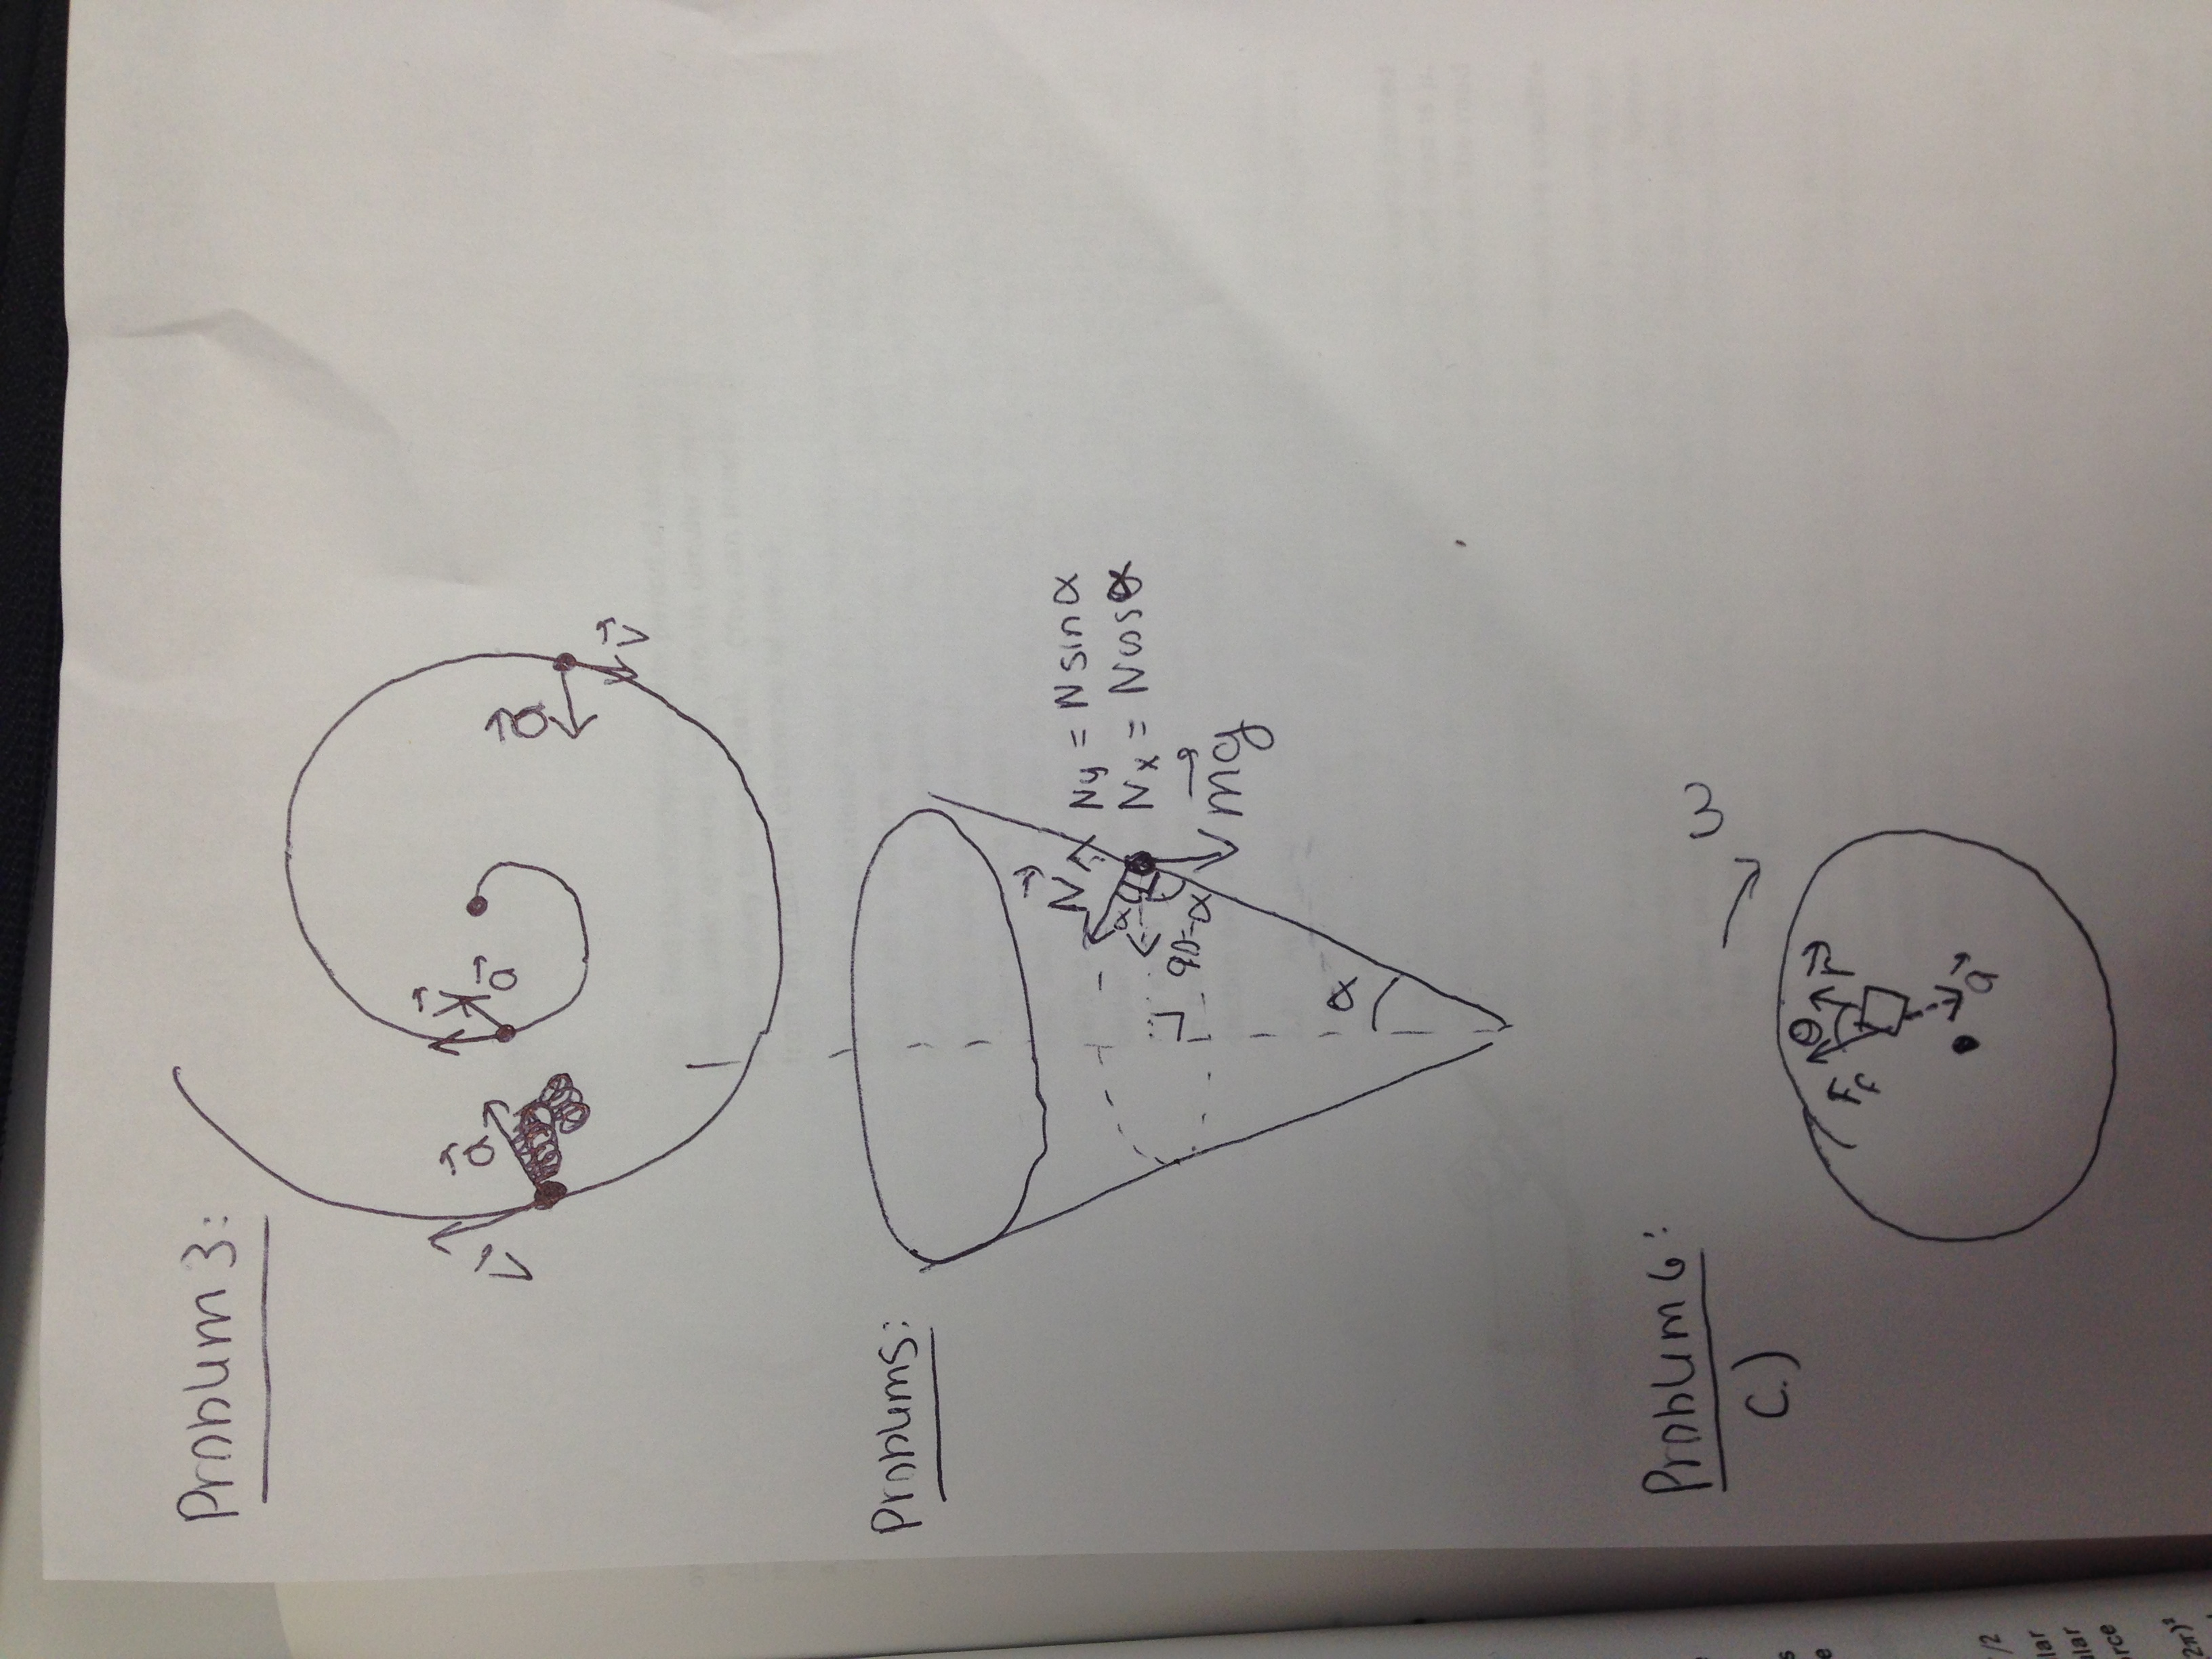
\includegraphics[width=1.4\textwidth,angle=270]{ps2.JPG}
\caption{The figures asked to be drawn in the problem set.}
\label{ps2}
\end{figure}

\end{document}



